%%%%%%%%%%%%%%%%%%%%%%%%%%%%%%%%%%%%%%%%%%%%%%%
\chapter{Scaffolding Citizen-led Knowledge Work}

\begin{quote}
\emph{This dissertation explores how the following things happen. Complex work is hard. Needs learning. People do things in groups. Social computing misses learning (learning is around but not here). why your title is what it is, what that means, how you set up your arguments, and what claims your introductory chapter makes.}
\end{quote}
\vspace{0.25in}

GI introduces a collaborative citizen science platform for people to transform lived exes into scientific theories

%people want to share info - see online fora  --have relevant images

Social computing (like digital photography) is a revolution: people can do more. Social computing platforms have enabled many things: sharing opinions, funding things, bringing down dictators. It has transformed how people share, discuss, and create insights. However, in its greatest successes, lie its terrible weakness. Social computing barely organizes people to perform personally meaningful work limited to experts: collective attempts to organize frequently fail, people create faulty insights from self-tracking, and more. Social media channels have given a greater loudspeakers to experts. In the absence of support and guidance, how can people do more. 

People possess a remarkable ability to identify patterns and create theories from their experiences. unfortunately, this is where they falter and don’t make any progress. How can we design systems that enable people to take these ideas and do more with them.

How can we think f social computing platforms that can effectively enable to do more personally meaningful work built upon their experiences and insights — to enable someone to find out whether drinking kombucha really changes the gut constitution, or to learn more about their microbiome based on what they’re eating without needing other external sources; in short, to push people towards actively testing their ideas rather than just sharing them.

This thesis explores integrating learning in social computing for complex, creative work with two main goals in mind: efficacy of the resulting systems (i.e. usability, correctness, and existential evidence) and generality of the underlying techniques upon which the tools are built.

Task-specific guidelines are used for review and other tasks, but existing idea offer limited ways for novices to create the artifact in the first place. Procedural training and reifying genre work is a new approach that enables people to do more. 


learning is not personal, work is not personal
People’s curiosity, needs, and possibilities to do useful work is endless; however, traditional online systems don’t support them. Online fora encourage long, rambling discussions. Online learning provides conceptual lessons but people drop out and these are not linked to people’s needs. Lack of appropriate "learning abstractions" make designing experiments (or any other scientific work) and performing xxx unrealistic — difficulty of managing all the different parts. 



2. hypotheses-testing
    1. novice inquiry systems
3. learning is not personal, work is not personal
    1. how do we integrate learning — we don’t know?
4. scientific motivation?
    1. this can also help inform new ideas that we are missing out on

People have strong personal motivations and contextual insights. To create knowledge, they need mental scaffolds for organizing complex work, domain knowledge to compose and execute the steps, and ways to ask for help. Experts benefit from conceptual knowledge, professional training, pre-existing organizational structure for collaboration, and direct access to resources. Currently, citizens lack these resources.How might online systems support citizen-led knowledge work? How can global communities create knowledge that meets their goals without waiting for experts to lead?

Supporting complex knowledge work has been a challenge for Human Computer Interaction research (make specific). For instance, many people are interested in understanding and improving their health. Millions of peple from all over the world share their insights 

Take experimentation, for instance. Despite a predetermined goal and a formalized process,
experimentation requires making contextually-appropriate
decisions [50]. Good experiment design is inherently user
centered; designers need awareness of others’ interpretation
of their ideas and asks. Providing feedback on experiment
designs requires knowing the success criteria and how to
help improve. Finally, successfully running an experiment
requires managing multiple processes such as random
assignment, anonymizing participant details, and sending
instructions and reminders for data collection.

Citizens have a different background than professional scientists; they have unique personal experiences
but lack the years of domain training. To create computational systems that leverage
their strengths and mitigate the lack of training, this dissertation focuses on domains where the science is nascent,
highly contextual, and personally motivating. Synthesizing the crowdsourcing literature and my
experience highlights three challenges: poor signal-to-noise from crowds due to lack of training;
inefficient collaboration without careful attention; and poor results (or no results at all) unless experts
lead. To address these concerns, my work introduces and evaluates peer production architectures
and procedural learning.

\begin{figure}[b] 
  \centering
  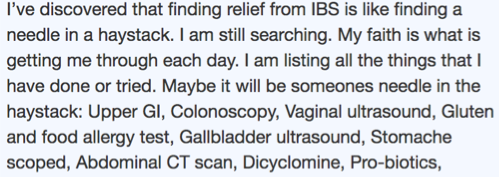
\includegraphics[width=1.0\textwidth]{figures/docent/fig-1.png}
  \caption[]
{This post to a Mayo Clinic forum shows how people
seeking advice online combine many ideas into one post..\index{docent-1}}
  \label{fig:docent-1}
\end{figure}


%%%%%%%%%%%%%%%%%%%%%%%%%%%%%%%%%%%%%%%%%%%%%%%%%%%
\section{Challenge: People' don't know what to do and how to do it}

poor signal-to-noise from crowds due to lack of training; inefficient collaboration without careful attention; and poor results (or no results at all) unless experts lead. To address these concerns, my work introduces and evaluates peer production architectures and procedural learning.

\textit{People lack the expertise to make situationally-appropriate choices}. 
Success with complex creative activities requires procedural
knowledge (how to do things) in addition to conceptual
knowledge (facts). While many resources offer facts, procedural
learning is often ignored.The converse also holds, and much more often: novices are also
“uninfected” by all the knowledge that enables experts to
innovate.

\textit{People lack a professional network to improve their work}. Furthermore, 

\textit{One more -- from docent and galileo}


how do we integrate learning in social computing?

\begin{figure}[h] 
  \centering
  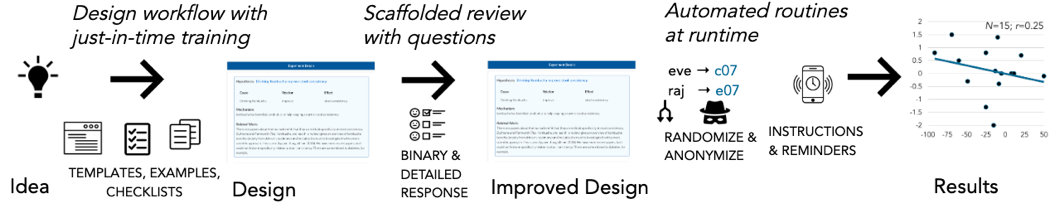
\includegraphics[width=1.0\textwidth]{figures/galileo/galileo-1}
  \caption[]
{Galileo enables anyone to design and run experiments to test their intuitions. Experiment creators can invite anyone to review and participate in the experiment. Participants from around the world join experiments, follow instructions, and provide data in response to automated data collection reminders.\index{galileo-1}}
  \label{fig:galileo-1}
\end{figure}

The central idea of this thesis is introducing learning in social computing for complex work. 
The thesis achieves this by building a sequnece of interactive prototypes that enable people in collaboratively generating hypotheses and experiments. Every protope advances social computing further as a domain for deep, personally meaningful work. 

\begin{figure}[b] 
  \centering
  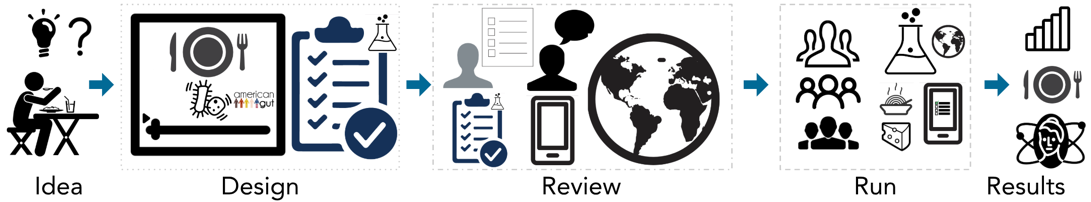
\includegraphics[width=1.0\textwidth]{figures/intro/intro-1}
  \caption[]
{The Gut Instinct platform enables anyone to transform their intuitions to hypotheses and then design and run experiments to test them [xx-xx]. Gut Instinct integrates conceptual learning embedded via short lectures and software-guided procedural learning to enable designing and reviewing experiments. Participants from around the world join experiments, follow instructions, and pro-vide data in response to automated data collection reminders. }
  \label{fig:intro-1}
\end{figure}

%%%%%%%%%%%%%%%%%%%%%%%%%%%%%%%%%%%%%%%%%%%%%%%
\section{Thesis: Procedural Support in Social Computing}


This dissertation explores challenges people face xxxxxxx. Underlying these investigations is the thesis:

//this is where you introduce the taxonomy 
//provide fig here from the research statement 

"My thesis statement is"
\begin{quote}
\emph{Integrating conceptual learning with task-specific scaffolding enables personally meaningful \& useful scientific work}
\end{quote}


%System contributions
“This thesis investigates the question: How to enable people to perform personally meaningful work that helps the world at large?”

To construct Gut Instinct, we framed the task of hypothesis-testing as a crowdsourcing problem, developed techniques and platform that supports different roles with just-in-time learning, and provided efficient backend support to automate simple tasks.

task with three elements: self-sourcing, crowdsourcing, and feedback 

%%%%%%%%%%%
\section{Contributions}
\begin{figure}[t!] 
  \centering
    \includegraphics[width=1.0\textwidth]{figures/img/intro/1-contributions}
  \caption[Contributions of this dissertation]
{Contributions of this dissertation including empirical results theoretical perspectives/techniques, real-world systems, and multiple outcomes}
  \label{fig:contributions}
\end{figure}

my work combines both interface design (expert systems) work with social computing 

This dissertation\textquotesingle makes two assumptions: 1) most people have an amazing breadth and depth of ideas , and 2) they lack the expertise to implement these ideas. Consequently, both people and the world lives in a severely sub-optimal space.

Two major issues in enabling complex work on the internet are (diversity and scale?) quality of individual contribution and the overall management of contributions.  We desire social computing techniques that reliably enable a wide variety of people to contrinute more than they naturally could and that manage the dependencies among a large set of tasks.

This dissertation\textquotesingle s primary contribution is the idea of intergrating learning in social computing to enable groups of novices to perform complex, creative task. To realize this idea, this dissertation makes three types of contributions: theoretical perspectives/techniques, real-world systems, and outcomes including empirical results, systems lessons, and dataset (Figure \ref{fig:contributions}). The techniques make the idea concrete; the system operationalizes the techniques and makes them work; and the outcomes discuss the successes and failures of our approach.

%todo - need terms for these


\subsection{Idea: Dual-objective online learning systems}
Dual objective systems have been around  a while. Commercial systems developed by Facebook and Google typically serve two purposes: provide a service to people (email, photos) and collect data; such data is used to train and improve Machine Learning algorithms, sold to third parties, and used for in-house advertising plans. While people receive the benefits of such technologies, it happens automagically.They don\textquotesingle 't learn anything.

My thesis proposes another future for dual objective systems --one where people perform work that is useful for others and the platform, but they also meet their needs. 
%add the system and people-led learning bits to social computing / crowdsourcing parts

\subsection{Theoretical: Techniques and Framework}
Improving the quality of work requires improvements at two levels: both the depth of work done per individual and the amount of work done overall. The former require better learning tools and the latter requires better collaboration tools and dependency management. 

Theoretical contributions include 1) principles to integrate learning in social computing, 2) User nterfaces and system design for efficient implementation", and 3) a characterization of the classes of activities that can work with this model.

\begin{itemize}
% come up with principles myself
\item Principles to integrate learning in social computing 
There are two kinds of learning: conceptual (declarative) and procedural. A large part of current education is about conceptual learning, where people learn what something is, learn about its features. Typically, such learning is tested with test questions. In contrast, procedural learning teaches the {\it how} of things. How do you do x, y, or z.  Concpetual learning is useful when xxx while procedural learning is more useful when yyy.

%figure about conceptual and procedural learning 

For useful contribution to complex work, people need to have a good working model of both the concepts and procedures for a thing. How does my dissertation deal with this?
1. reify conceptual bits in the software itself or provide via video //
2. Drawing from learning psychology and not attention psychology 
-- see the ethical engineering award thing
3. 

The efficacy of these techniques is borne out over multiple deployments. 

\item  Principles to decompose Complex work to f(people, community, \& machines)
% figure -- def needs one -- based on strengths and weaknesses

Social computing relies on carefully designing the affordances, support, and system to enable different users for different needs.

1. The individual, a group, and groups of machines possess complementary strengths. \\
Individual: creative, lived experience gives ideas, personal context, creative, willing to push through \\
community: lesser motivation but willing to help (diff roles to contribute), another set of eyes, diverse ideas --> check biases \\
machines: consistent implementation, reduces biases
(see slide deck)

2. Think of complex work as simpler tasks where the system manages the interdependencies

proof: success of the experimentation platform

\end{itemize}

All these techniques have been put in systems as interfaces, intelligent backends, and so on... \\
//present a stack of things

\subsection{System Design (including Interfaces)}
%%"Furthermore, adding location information to photo collections is by itself insufficient for scenevisualization: we also need intuitive, interactive interfaces for exploring these scenes. There are several challenges faced in the design of such interfaces. First, unlike with Google Street View, where photos are taken at regular intervals, personal or Internet collections are typically an unstructured soup of photos. Nevertheless, the navigation controls should still be intuitive and exhibit regularity. Second, such controls should make it easy to find and explore the interesting parts of a scene, particularly for tourist sites."


Furthermore, providing techniques is not enough. 

The techniques described above need to be implemented in ways that are easy to understand, access, and use for most people. This happens by baking these in the user interface (which is the direct thing people interact with) and by building a backend that is based on the principles of x, y, and z.

\subsubsection{User Interfaces}
\begin{itemize}
\item UIs that implement learning ( conceptual + procedural)
\item UIs for focused collaboration  
\end{itemize}

\subsubsection{System design}

\begin{itemize}
\item system-led learning vs people-led
\item Backend that manages the task dependency, and transparency among users
--- finite state machine (history of...)
--- drawing from parser, compiler + lex/yacc format for this state machine for complex tasks ideas
\item  db optimizations
\end{itemize}

state diagram — the edges represent what people need to do 

\subsubsection{Roles Support via Just-in-time Skill Acquisition}
 People take different roles
--write up form galileo


%%%%%%%%%%%%%
\subsection{Outcomes}
\subsubsection{Empirical Results from Real-world Deployment}
expertise: limited; diversity: different countries; scale: some

\subsubsection{Lessons}
\begin{itemize}
\item improved methods to test usability of my systems and techniques -- via multiple deployments
\item xxx
\end{itemize}

\subsubsection{Dataset}
1. repo of hypotheses with rating
2. repo of experimental designs
3. ...

\section{Impact}
 \subsection{Used by communities}
 \subsection{Talks in the Research community and other communities}
 \subsection{Taught in classes}

%%%%%%%%%%%%%%%%%%%%%%%%%%%%%%%%%%%%%%%%%%%%%%%%%%%%%%%%%%%%
\section{Opportunity: Harnessing humanity\textquotesingle s collective efforts accomplishes great goals}


\textit{People have complementary knowledge in comparison to experts and are uninfected by expert biases}
--drawn from lived experience
-- individually and collectively

Sometimes, having a different background than experts can
be beneficial. Shared knowledge is great when it’s right, but
blocks progress when wrong. When false assumptions limit
experts, at least some novices are likely to be “uninfected”.
For example, GalaxyZoo volunteers discovered ‘green pea’
galaxies overlooked by scientists who mistakenly assumed
the green hue was merely an imaging artifact [54]. 

\textit{Learning resources proliferate and people learn from personal interest/hobby but it's not directly linked to their personal thing}
Creative, open-ended work has rich pedagogical value.
Online work, like online learning, requires appropriate
scaffoldings, such as rubrics [12,41], decision trees [43,57],
tutorials [6], and quick expert guidance [23]. Similar to
general critique of pure discovery learning [47], simply
asking participants to “figure it out” would be poor pedagogy. Hence, Gut Instinct introduces a guided discovery
learning approach as Mayer advocates: expert-curated
learning materials help participants start, with discovery
following. Recruiting learners as citizen scientists offers a
Problem-based Learning experience with context and motivation for the material students learn [50]. In principle,
these real-world problems also provide a yardstick for
measuring learning. 

\textit{Second-order effect: People are connected online and collectively have access to many resources}
In a large distributed community, there’s often
someone who happens to have important relevant
knowledge, usually drawing on a relevant but distant domain. Such distributed efforts are a type of lead-user innovation [31]. Having many people work on the same problem increases the odds that one will break through. Drawing
on secondary expertise as inspiration can be an important
agent of creativity because almost by definition, the combination is rare [10]. Open \& crowd innovation builds up on
contributions by diverse online participants, and a ‘bubbling
up’ process for strong ideas [56].


from the talk
1. People design, build, and track to better understand and improve their health
    1. Dana Lewis work
2. Worldwide, people use online health fora to share insights and look for answers
    1. On numerous online fora, people share their intuitions, observations, folk theories, and even results from trying different approaches to improve their health, e.g. from simple ideas like ‘giving up drinking coffee to improve quality of sleep’ to tests and dietary approaches. 
3. People draw ideas from current research by reading and discussing papers
    1. Shouldn’t we tie the to the scientific community? but how?
    2. In many cases, these discussions are not just anecdotal but also derive from state-of-the-art scientific work.
    3. In some cases, people contribute back to scientific work as well
4. introduce lead users
    1. “Lead users are rarely experts by themselves. They are novices who find themselves at the right place, with the right tools (that they might have created themselves), and who have the courage to follow through.”
    2. Lead users have created different—and in some cases better designs— than experts 
5. Citizens have successfully solved expert-defined problems as sensors or algorithms
    1. For long, citizen scientists have been amateurs who contribute scientific work - typically
        1.  under the guidance of experts 
        2.  on large projects
        3.  that are intractable with existing scientific resources.
    2. citizen science for long has continued work with this row-filling model of contribution rather than providing a truly independent, participatory experience. 
6. dual nature
    1. Science can answer life-relevant questions 
but few know how to even get started
    2. Institutional science misses out on ideas from beyond the ivory tower
7. goal
    1. Environments for learning and collaboration through complex, personally meaningful work

from papers
1. Scientific experimentation features technical requirements and contextual choices that are inscrutable for a lay individual yet necessary for success [50]. While professional scientists and commercial ventures run experiments every day, with notable exceptions [15,47], empirical papers from non-professionals are vanishingly rare. This biases the questions asked, studies run, and knowledge created [18,31]. People have questions about their health, but lack the expertise and resources to scientifically investigate them. Broadening the pool of experimenters could help people investigate their curiosities, develop solutions to improve health and performance, and assist institutional researchers.
2. 

My research advances the design of social computing systems by integrating learning and collaborationto enable complex work such as generating and evaluating scientific theories. Over 600 people from 30 countries have self-organized to generate theories about the human microbiome and test them by running experiments. My research raises the question: how can global communities create knowledge that meets their goals without waiting for experts to lead? My research prototypes collective systems for large-scale problems.

My doctoral research demonstrates how we might draw on people’s diverse backgroundknowledge, interest, and micro-expertise to expand scientific knowledge and push it in new directions. More specifically, the Gut Instinct platform that I have built instantiates these ideas enabling participants of the American Gut Project (the world’s largest crowdfunded citizen science project) to generate and experimentally investigate hypotheses (Figure 1). 344 volunteers from 27 countries created 399 hypotheses about their health and the gut microbiome. Remarkably, microbiome scientists rated a fifth (75) of these hypotheses to have a scientifically valuable insight about a topic not covered by existing published work. Volunteers fleshed out 60 of these hypotheses into complete experimental designs. My entire work (code + data) is open source so others can edit, build, and experiment.

Many hands make light work, but novices needclear contribution opportunities The crowdsourcing literature offers many good verification approaches for tasks with clear right or wrong answers – like whether two images represent the same product or what street number is written on a sign. However, verifying knowledge work necessitates a different approach because it requires making situationally-appropriate choices. Gut Instinct divides multi-party collaboration into complementary tasks and supports them using different contribution mechanisms (like adding a question, editing a response) and roles (like experimenter, reviewer, participant). This provides people the flexibility to choose how much they’d like to contribute. Finally, Gut Instinct automatically manages multiple activities to reduce bias and experimenter/participant workload,such as randomized placement of people into conditions, maintaining anonymity, and collecting and cleaning data.


%%%%%%%%%%%%%%%%%%%%%%%%%%%%%%%%%%%%%%%%%%%
\section{Dissertation Roadmap}

%%%%%%%%%%%%%%%%%%%%%%%%%%%%%%%%%%%%%%%%%%%%%%%%%%%%%%%%%%%%%%%%%%
%todo- “we” refers to the set of authors…  -- see arvind


"double quotes"

